\documentclass{specification}
\usepackage[backend=bibtex]{biblatex}
\usepackage{dsfont}
\usepackage{graphicx}
\usepackage{epstopdf}
\usepackage{booktabs}
\usepackage{csquotes}
\bibliography{bibliography}


\title{Automated Protein Function Description for Novel Class Discovery}
\author{Meet Barot}

\begin{document}

\maketitle

% How many citations do NEURIPs workshop papers have? Have that many at least.
\section{Abstract}
%High-throughput sequencing technologies have allowed us to amass millions of protein sequences from organisms throughout the tree of life.
Knowledge of protein function is necessary for understanding biological systems, but the discovery of new sequences from high-throughput sequencing technologies far outpaces their functional characterization.
Beyond the problem of assigning newly sequenced proteins to known functions, a more challenging issue is discovering novel protein functions.
The space of possible functions becomes unlimited when considering designed proteins.
Protein function prediction, as it is framed in the case of Gene Ontology term prediction, is a multilabel problem with a hierarchical label space.
However, this framing is limiting. It does not provide guiding principles for discovering completely novel functions.
Clustering-based approaches are not able to give much information about the new functional categories that they predict; they can only predict that a protein may belong to a category that has not been studied.
In this work we propose a neural machine translation model in order to generate descriptions of protein functions in natural language.
We provide quantitative results of our model in the zero-shot classification setting, scoring functional descriptions that the model has not seen before, as well as function descriptions for qualitative evaluation.

\section{Introduction}

    \subsection{Motivation}
    Why make a model that describes the common functions of a set of proteins in natural language?
        \subsubsection{Sets as input.}
            We describe protein function as abstractions of what we know groups of proteins to do. This is a more general way of framing the problem that matches the way the GO terms themselves were created. % back this statement up a bit, probably from GO paper
        \subsubsection{Natural language output.}
            We want to be able to describe proteins in a compositional way, so that we have the ability to describe any set of proteins given to the model. This gives us an ability to describe functions that have not been characterized already for free, rather than having to train a new model or rely on specific examples of that function.
        \subsubsection{New function discovery.}
            We want to be able to predict the functions of proteins, but we are limited by the amount of data that we have in both the amount of well characterized proteins and also the variety of known functions. Even the best supervised approaches can only take us to the point where we can annotate proteins that have functions that have been seen before.
        \subsubsection{Existing approaches do not give testable hypotheses.}
            Explicitly ontology-based zero-shot approaches such as DeepGOZero \cite{DeepGOZero} do not allow for actual description of a new function that is discovered.
            The only information that is gained is that the protein has a new function that has some specified ontological relation to currently known functions.
            However, this may not sufficiently describe the new function, and it also excludes possible functions that do not directly relate to known functions.
            In order to discover new categories of protein function, with some amount of information to actually design experiments to test for them, we need a model that generates functional descriptions.

\section{Related Work}
\subsection{Protein Function Prediction} % Probably need to update this, search for new function discovery methods.
Many methods have been proposed for protein function prediction, though most do not consider the problem of discovering novel functions.
Instead, the task is generally framed as a supervised multilabel problem where the predicted labels are all assumed to have some example in the training set.
Yet most unlabeled proteins, especially in understudied organisms, are likely to perform functions that have not yet been characterized.
The supervised approach does not address this possibility, and so new methods must be proposed for function discovery.

Clustering-based approaches are not able to give much information about the new functional categories that they predict.
They can only predict that a protein may belong to a category that has not been studied.
One could compute average distances to clusters that contain known proteins, but beyond this, there is no testable hypothesis that the model can give about their function.

Zero-shot learning approaches attempt to address the unseen class problem as well, mostly by creating continuous embeddings of the labels and predicting a mapping from the input to real-valued vectors in that learned label space \cite{CLIP}.
Similar to clustering-based approaches, not much information about the unseen class is gained besides its distance from existing categories and its direction in the abstract label space.
DeepGOZero \cite{DeepGOZero} is a method that uses ontology axioms to predict for classes with no examples in the training set.
However, the classes that are able to be predicted must be defined with ontological relations to seen classes.
This constraint both restricts the possible novel functions that can be discovered and may not give sufficient information to design an experiment to test for the novel function.
Among the few zero-shot approaches proposed for function prediction, none are able to describe the novel functions discovered in natural language.

\subsection{Neural machine translation}

\section{Methods}
\begin{figure}
    \centering
    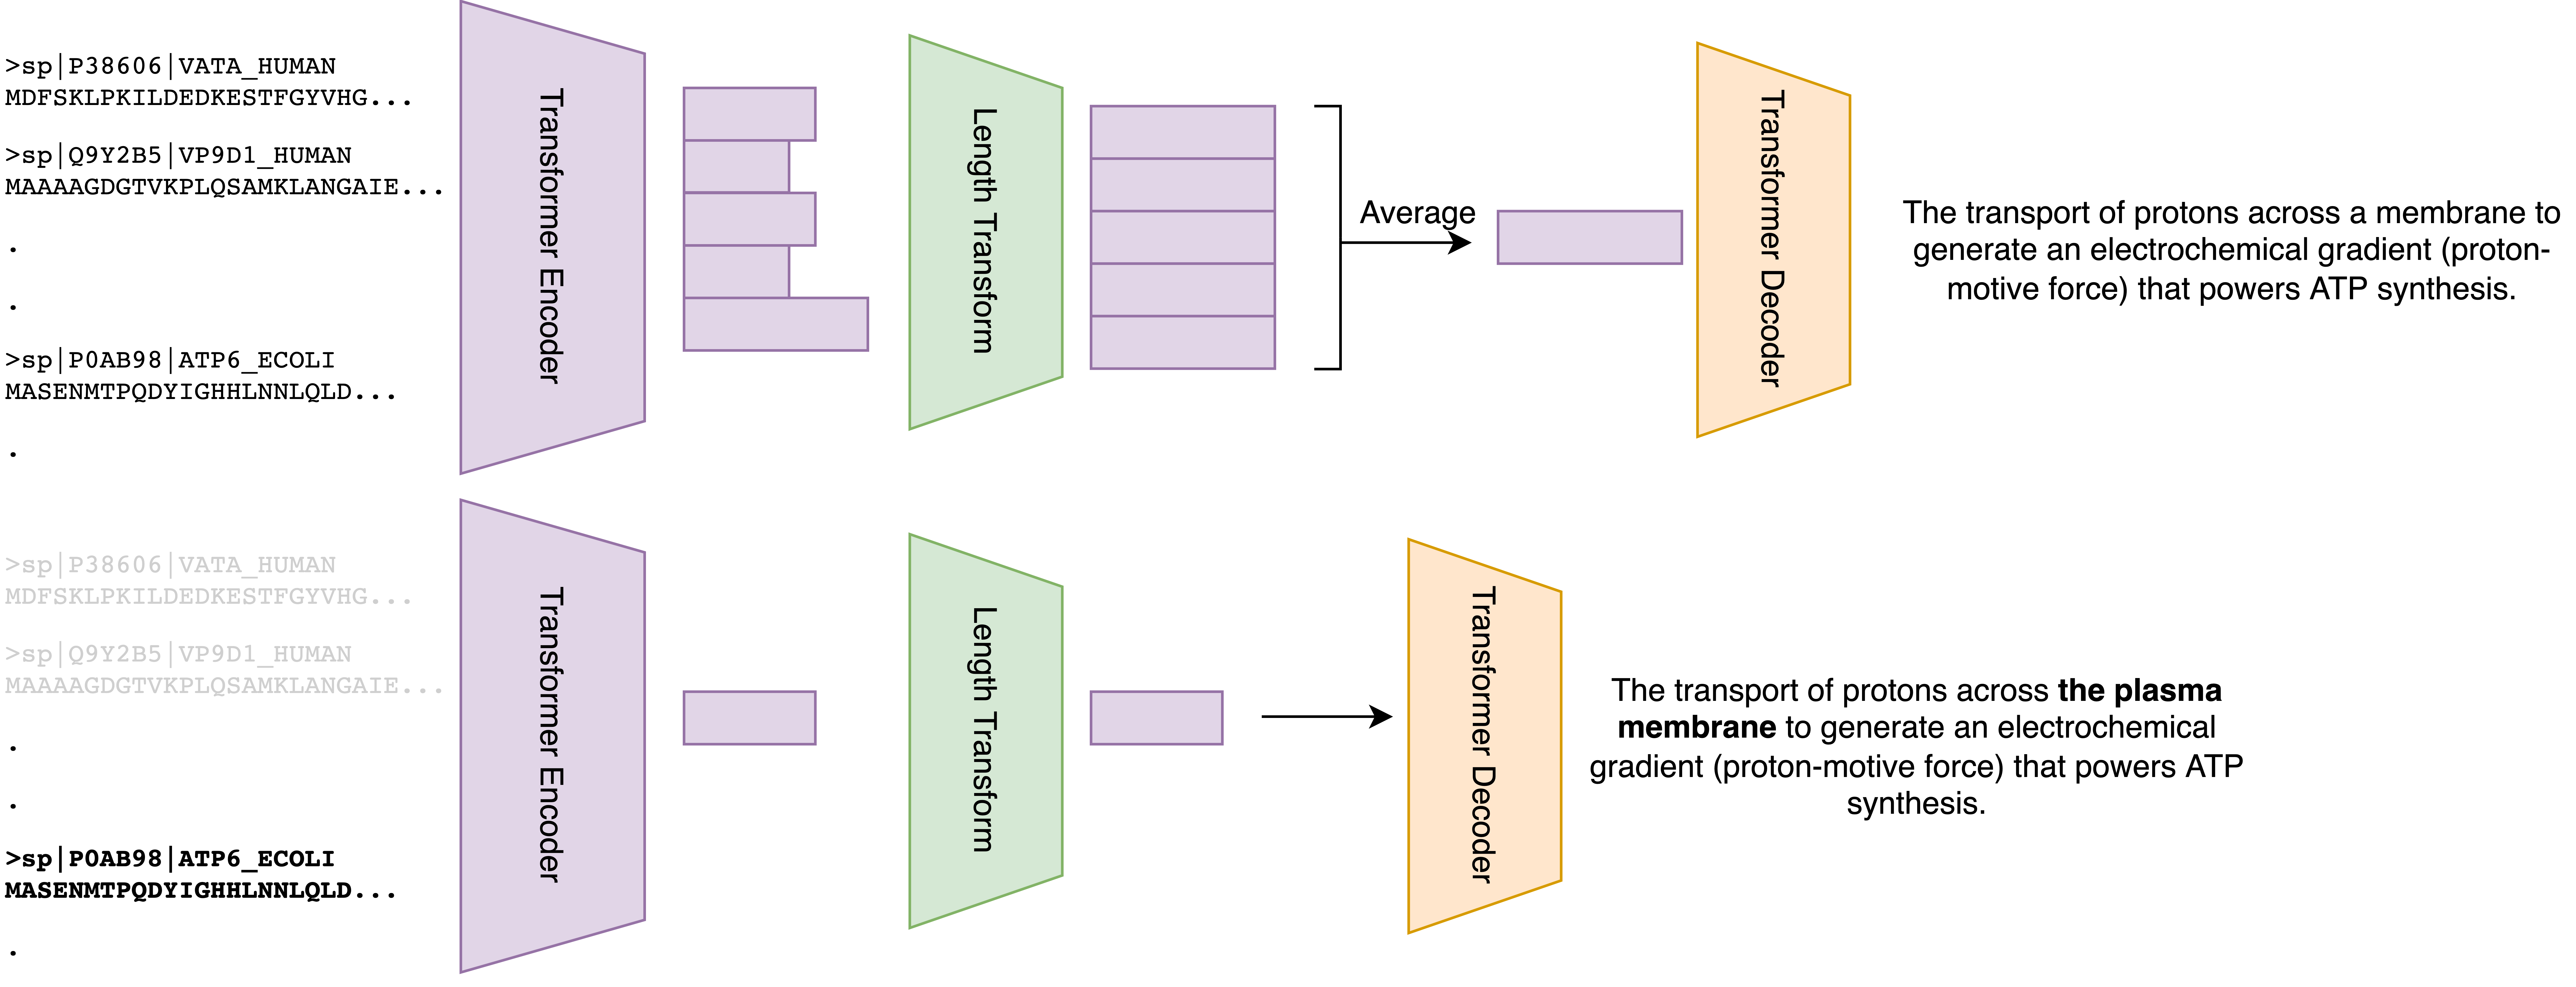
\includegraphics[width=0.9\linewidth]{prot2go.png}
    \caption{High-level diagram of the proposed transformer encoder-decoder model.
The model is trained to produce the most specific common function of the input protein sequences.}
    \label{overview}
\end{figure}
    \subsection{Permutation invariance of protein sets to describe}
    We begin describing our method with the way we construct our input. We use sets of protein sequences, invariant to ordering, as input to the model giving a description. In this way, we are making the problem more general: our task is to describe the function of a set of any number of proteins. This matches the manual process of characterizing new functions. Biologists describe and categorize functions which are abstractions of the common behavior of groups of proteins in nature, so we want our model to be able to perform this abstraction given any set of proteins.
    \subsection{Autoregressive generation of descriptions}
    Another contribution we make in proposing this method is to generate protein function descriptions in natural language. This allows for the characterization of proteins in a compositional way, with a grammar such that all protein sets can be described with the model, not just those with particular sets of terms the scientific community has manually assigned with the Gene Ontology.
    \subsection{Transformer encoder-decoder model}
    We use a transformer encoder-decoder model \cite{vaswani2017attention} with a length transform \cite{shu2020latent} to handle differing sequence lengths in order to average sequence features from the encoder.
    \subsection{Length transform}
    The model takes sequences of varying length. The sequences' representations should be combined in some way that preserves the amino acid ordering. We use the length transform in order to shape the representations such that they can be combined while order information is preserved.
    \subsection{Zero-shot Classification setting}
    Fundamentally, our model assigns probabilities to pairs of protein sets and descriptions. In order to evaluate the method, we use the zero-shot classification setting, where we wish to classify proteins into unseen categories. We develop three metrics in the Evaluation section to evaluate the distribution learned by the model in this classification setting.

    \subsection{Generation (beam search)}
    Generation of descriptions is a search problem through the set of all possible output token sequences, where the goal is to find the sequence with the largest probability. Generation given an autoregressive model is a highly studied problem in the natural language processing literature.% cite a review paper on language model generation methods
    We use beam search in the current implementation in order to find reasonable generated descriptions. Evaluation of these descriptions is an unsolved problem; currently, manual inspection by expert human evaluators is the best method we have.
\section{Evaluation}
In this section, we define three metrics that can be computed using known functional descriptions in order to evaluate our models' learned probability distributions.

Generated descriptions are shown in the Results section for qualitative analysis.
Quantitative analysis of the generated descriptions requires data from human evaluators with expertise in protein function in order to determine the accuracy of generated descriptions.
A framework for performing that analysis with expert curators is explored in the Discussion section.
    \subsection{Metrics}
        \subsubsection{Attribute 1: Annotation correctness.}

        Given a sequence set for which the model is assigning scores to function descriptions, descriptions of GO terms that annotate the entire sequence set should be scored higher than terms that do not annotate the entire sequence set.

        Let $D_{S}$ be the GO term descriptions associated with sequence set S.

        \[P(d \in D_{S} | S) > P(d \notin D_{S} | S)\]

        A way to measure this attribute would be to calculate:
        \[\frac{1}{|D_{S}|*|D_{S}^{c}|}\sum_{d_i \in D_{S}, d_j \notin D_{S}} \mathds{1}(P(d_i | S) > P(d_j | S))\]
        where $D_{S}^{c}$ is the complement of $D_{S}$ and $\mathds{1}$ is the indicator function.

        \subsubsection{Attribute 2: Specificity preference.}

        Among terms that do annotate the whole set, the model should score child terms higher than their ancestor terms.
Let $A(d)$ denote the description of a direct parent of the GO term described by $d$.

        \[P(d \in D_{S}| S) > P(A(d) \in D_{S}| S)\]
        Note: any protein set that is annotated with $d$ would always be annotated with $A(d)$, $A(A((d))$ and so on.

        A way to measure this attribute would be to calculate:
        \[\frac{1}{|D_{S}|}\sum_{d_i \in D_{S}} \mathds{1}(P(d_i | S) > P(A(d_i) | S))\]

        \subsubsection{Attribute 3: Annotation robustness.}

        Any set of sequences that have the same exact set of GO descriptions in common should be scored with the same rankings for those GO descriptions.

        Let $S_i$ and $S_j$ be different sequence sets such that $D_{S_i} = D_{S_j}$ and $S_i \neq S_j$, and let $R(X)$ be a ranking function that gives the ranks of entries in $X$, in descending order.

        \[R_{d}(P(d \in D_{S_i} | S_i)) = R_{d}(P(d \in D_{S_i} | S_j))\]

        A way to measure this attribute would be to calculate the average Spearman's rank correlation of the rankings for all sequence sets' correct descriptions.
Let $R_{S_i} = R(P(D_{S_i} | S_i))$:

        \[\frac{1}{N*(N-1)}\sum_{S_i, S_j} \frac{\textnormal{cov}(R_{S_i}, R_{S_j})}{\sigma_{R_{S_i}}\sigma_{R_{S_j}}}\]

        where $N$ is the total number of sequence sets that have the exact set of GO descriptions $D_{S_i}$.
In reality, this number may be too large to actually sum (especially if $|D_{S_i}|$ is small), so we approximate this measure by subsampling $n < N$ sequence sets to average over instead.
The sum is only calculated over non-identical pairs of sequence sets.

\section{Data}
We take sequences and annotations from the Uniprot-KB Swiss-Prot database, which is manually annotated and reviewed, in order to create our training and evaluation sets of proteins and function descriptions. This database had 566,996 proteins total. To focus on the functions that were both specific enough and had a sufficient number of examples in our evaluation sets, we restricted the maximum number of proteins per GO term to 1280, and minimum number of proteins to 32. The number of proteins and GO terms that were used in our training set as well as different evaluation sets are listed in Table \ref{tab:datasets}.
\begin{table}
    \caption{Number of proteins and GO terms in training and test sets.}
	\centering
	\begin{tabular}{c|cccc}
		\toprule
         & Train P\&F & Train P, Test F & Test P, Train F & Test P\&F \\
		\midrule
        Prots & 316k & 181k & 20k & 20k \\
        Funcs & 9k & 2k & 879 & 1.5k \\
		\bottomrule
	\end{tabular}
	\label{tab:datasets}
\end{table}

\section{Results} % Need to see the naive performances that Kyungyhun suggested to compare to
\begin{enumerate}
    \item Plots of the models with the three metrics.
Training proteins with training GO terms, test proteins with training GO terms, and test proteins with test GO terms.
    \item Analysis of what differences the models have in terms of architecture or training, and how that relates to the difference in performances across the three measures and the three settings of function prediction:
        \begin{enumerate}
            \item Train set proteins/functions
            \item Proteins part of test set but with train set functions
            \item Proteins part of test set with test set functions
        \end{enumerate}
    \item Table of randomly selected generated descriptions of protein sets that have GO terms not in the training set for each model. % have some, is it enough?
    \item Perhaps some analysis of the model's performance with respect to point anomalies, contextual anomalies, group anomalies? Would likely need to create specific datasets for these tests % probably too much for workshop paper
\end{enumerate}

        We show model performances in Table \ref{tab:performances}. The table suggests that the model is able to rank uneen functions for protein sets that it has been exposed to in training, with the model's rankings of identically annotated sets being in moderate agreement. For test proteins that have less than 30\% sequence identity to the training set, the model is still able to assign rankings of 1000 randomly selected functions from the training set with a correctness 30\% above random assignment (0.5). For the low-similarity test proteins that have functions that are not seen in the training set, the model is still able to rank 21\% better than random rankings.

        Although the performance is not very high compared to most protein function prediction methods for unseen proteins, we are mainly focused on using the model for generation, and these metrics are meant mostly as guides for model design. The loss function used is not optimizing for classification accuracy; it is optimizing the model's probability distribution to assign high probability to descriptions assigned to a sequence set.

        We show sample test set descriptions in Table \ref{tab:descriptions}. The left column is a GO description that annotates a sampled sequence set and the right column is the models' generated description of that sequence set. The first row shows that the model describes verbatim a related term (GO:0001654, eye development) for the proteins selected. Their common ancestor term is anatomical structure development (GO:0048856). This description is more specific than the actual term from which the proteins are sampled, but the description is wrong. The next generated description is more general than the actual description of the sampled set (modulates vs. activates), but is correct; it is the direct parent of the true term. The third generated description is related but ultimately different than the actual description of the protein set. The fourth generated description is more specific than the true common GO description of the set; it is a descendant term.
\begin{table}
	\caption{Model Performances}
	\centering
	\begin{tabular}{l|llll}
		\toprule
        Metric & Train P, Test F & Test P, Train F & Test P\&F \\
		\midrule
        Annotation Correctness & 0.8844 & 0.8014 & 0.7157 \\
        Specificity Preference & 0.5765 & 0.5526 & 0.5701 \\
		Annotation Robustness & 0.4020 & 0.1977 & 0.2362 \\
		\bottomrule
	\end{tabular}
	\label{tab:performances}
\end{table}
\begin{table}
	\caption{Sample Test Set Description Generations}
	\centering
    \begin{tabular}{p{8 cm}|p{8 cm}}
		\toprule
        True Common GO Description of Sequence Set & Model Generated Description of Sequence Set \\
		\midrule
        <SOS> the process in which the anatomical structures of appendages are generated and organized . an appendage is an organ or part that is attached to the trunk of an organism . <EOS> & <SOS> the process whose specific outcome is the progression of the eye over time , from its formation to the mature structure . <EOS> \\ \hline
        <SOS> any process that activates or increases the frequency , rate or extent of cell differentiation . <EOS> & <SOS> any process that modulates the frequency , rate or extent of cell differentiation . <EOS> \\ \hline
		<SOS> a protein complex that contains the gins complex , cdc45p , and the heterohexameric mcm complex , and that is involved in unwinding dna during replication . <EOS> & <SOS> any process involved in forming the mature 3 ' end of a dna ( mrna ) molecule . <EOS> \\
        \hline
        <SOS> the targeting and directed movement of proteins into a cell or organelle . not all import involves an initial targeting event . <EOS> & <SOS> the directed movement of proteins from endoplasmic reticulum to the nucleus . <EOS>  \\
		\bottomrule
	\end{tabular}
    \label{tab:descriptions}
\end{table}
%\begin{table}
%	\caption{Description Generation}
%	\centering
%    \begin{tabular}{p{7.5 cm}|p{7.5 cm}}
%		\toprule
%        True GO Description & Generated Description \\
%		\midrule
%        binding to fructose 6-phosphate . & catalysis of the reaction sinapaldehyde + nadph = nadp+ = h+ . \\ \hline
%        catalysis of the reaction n6- ( 1 , 2-dicarboxyethyl ) amp = fumarate + amp . & catalysis of the reaction 2-deoxy-d-ribose 5-phosphate = d-glyceraldehyde 3-phosphate + acetaldehyde + acetaldehyde + acetaldehyde ... \\ \hline
%		the chemical reactions and pathways involving of salicylic acid ( 2-hydroxybenzoic acid ) , a derivative of benzoic acid . & the chemical reactions and pathways resulting in the formation of asparagine , the fundamental heterocyclic group of asparagine , from simpler precursors , the formation of the formation of the formation of the formation of the multisubunit water-soluble proteins , the formation of the multisubunit water-soluble proteins , the multisubunit water-soluble proteins , the multisubunit water-soluble proteins , the formation of the formation of the formation ... \\
%		\bottomrule
%	\end{tabular}
%\end{table}


\section{Discussion}
In this work, we have proposed a novel method to generate protein function descriptions in order to discover new protein functions.
We have demonstrated that our model can accurately rank unseen function descriptions for proteins not seen in the training set, and show promising results in generated function descriptions.
Below, we explore how we might further evaluate the method's generated descriptions using human expertise and curation.

\subsection{Future human-assisted evaluation of function discovery}
As our scoring metrics for evaluation are automated, they can be used for optimizing the architecture and other hyperparameters of the model (either manually or with some search method).
However, in the case of actual use on proteins that are not very well studied, it can be difficult to know whether a given description is accurate.
Human-assisted evaluation will be needed for the descriptions generated for a given set of novel proteins.
This feedback could be used to fine-tune the model to produce more accurate, fluid or generally desirable descriptions of proteins, as has been done for document summarization models \cite{finetuningWithHuman, learningToSummarize}.

One possible way of obtaining human feedback would be to ask an expert with knowledge of the Gene Ontology and familiarity with some families of proteins to choose between two descriptions for a given sequence set that is generated from a trained model.
Doing this over a large enough dataset would allow us to train a reward estimation model that can then be used to fine-tune the original trained model using reinforcement learning.
However, this would be expensive, as the task needs to be done by an expert.
Richer information, such as ranking the similarities to an existing GO term, or suggesting changes to particular portions of the description, could be used to increase performance even with a small number of examples with human feedback.

% need a concluding statement
\printbibliography

\end{document}
